\documentclass[a4paper,12pt]{article}
\usepackage[spanish]{babel}
\usepackage[utf8]{inputenc}
\usepackage{booktabs}
\usepackage{dirtytalk}
\usepackage{graphicx}
\usepackage{makecell}
\usepackage{listings}
\lstdefinestyle{myCustomMatlabStyle}{
  language=C,
  tabsize=3,
  showspaces=false,
  showstringspaces=false
}

\begin{document}

\title{\Large Instituto Politécnico Nacional\\Escuela Superior de Cómputo\\Análisis de algoritmos\\Práctica 2: Métodos de Búsqueda\\Alumno: Meza Zamora Abraham Manuel}
\date{}
\maketitle

\section{Resultados obtenidos }
El arreglo utilizado en las funciones es el siguiente:\\
\begin{table}[h]
\centering
\begin{tabular}{ | c | c | c | c | c | c | c | c | c | c |  c | c | c | c | c | c | c | c | c | c | }
\hline
1 & 2 & 3 & 4 & 5 & 6 & 7 & 8 & 9 & 10 & 11 & 12 & 13 & 14 & 15 & 16 & 17 & 18 & 19 &  20\\
\hline
\end{tabular}
\end{table}

\begin{enumerate}
\item Búsqueda secuencial
\begin{itemize}
\item Función
\\ \lstset{basicstyle=\tiny,style=myCustomMatlabStyle}
\begin{lstlisting}
void busqueda_secuencial(int *arreglo, int tam, int num_a_buscar)
{
        int i, bandera = 0;
        for (i = 0; i < tam && bandera == 0; i++)
                if (num_a_buscar == arreglo[i])
                        bandera = 1;
        if (bandera == 0)
                printf( "No se encontro el numero %d en el arreglo\n", num_a_buscar);
        else
                printf("Se encontro el numero %d en el la posicion %d, en %d pasos.\n"
                , num_a_buscar, i - 1, i);
}
\end{lstlisting}
\item Resultado obtenido.
\\ \lstset{basicstyle=\tiny}
\begin{lstlisting}
BUSQUEDA SECUENCIAL
Se encontro el numero 1 en el la posicion 0, en 1 pasos.
Se encontro el numero 10 en el la posicion 9, en 10 pasos.
Se encontro el numero 20 en el la posicion 19, en 20 pasos.
No se encontro el numero 880 en el arreglo
\end{lstlisting}
\end{itemize}
\item Búsqueda binaria
\begin{itemize}
\item Función

\lstset{basicstyle=\tiny}
\begin{lstlisting}
void busqueda_binaria(int *arreglo, int tam, int num_a_buscar)
{
        int i = 0, j = tam - 1, m, pasos = 0, bandera = 0;
        while (i <= j && bandera == 0)
        {
                m = i + (j - i) / 2;
                if (arreglo[m] == num_a_buscar)
                        bandera = 1;
                if (arreglo[m] < num_a_buscar)
                        i = m + 1;
                else
                        j = m - 1;
                pasos++;
        }
        if (bandera == 0)
                printf("No se encontro el numero %d en el arreglo\n", num_a_buscar);
        else
                printf("Se encontro el numero %d en el la posicion %d, en %d pasos.\n"
                , num_a_buscar, m, pasos);
}

\end{lstlisting}

\item Resultado obtenido.

\begin{lstlisting}
BUSQUEDA Binaria
Se encontro el numero 1 en el la posicion 0, en 4 pasos.
Se encontro el numero 10 en el la posicion 9, en 1 pasos.
Se encontro el numero 20 en el la posicion 19, en 5 pasos.
No se encontro el numero 880 en el arreglo
\end{lstlisting}

\end{itemize}
\item Árbol de búsqueda binaria

\begin{itemize}
\item Función 

\begin{lstlisting}
Nodo* buscar(Nodo* raiz, int dato, int* pasos)
{
        int encontrado = 0;
        while (!encontrado && raiz != NULL)
        {
                *pasos += 1;
                if (dato == raiz -> numero)
                        encontrado = 1;
                else if (dato < raiz -> numero)
                        raiz = raiz -> izquierdo;
                else if (dato > raiz -> numero)
                        raiz = raiz -> derecho;
        }
        return raiz;
}
\end{lstlisting}

\lstset{basicstyle=\tiny}
\begin{lstlisting}


void buscar_Arbol(Nodo *raiz, int num_a_buscar)
{
        int pasos = 0;
        if(!buscar(raiz,num_a_buscar,&pasos))
                printf("No se encontro el numero %d en el arbol, 
                se dieron %d pasos.\n", num_a_buscar, pasos);
        else
                printf("Se encontro el numero %d en el arbol, se dieron %d pasos.\n"
                , num_a_buscar, pasos);
}

\end{lstlisting}

\item Resultado obtenido:

\begin{lstlisting}


BUSQUEDA Arbol cargado a la izquierda
Se encontro el numero 1 en el arbol, se dieron 20 pasos.
Se encontro el numero 10 en el arbol, se dieron 11 pasos.


BUSQUEDA Arbol Balanceado
Se encontro el numero 20 en el arbol, se dieron 5 pasos.
No se encontro el numero 880 en el arbol, se dieron 5 pasos.

\end{lstlisting}

\end{itemize}

\end{enumerate}

\center
\begin{figure}[h]
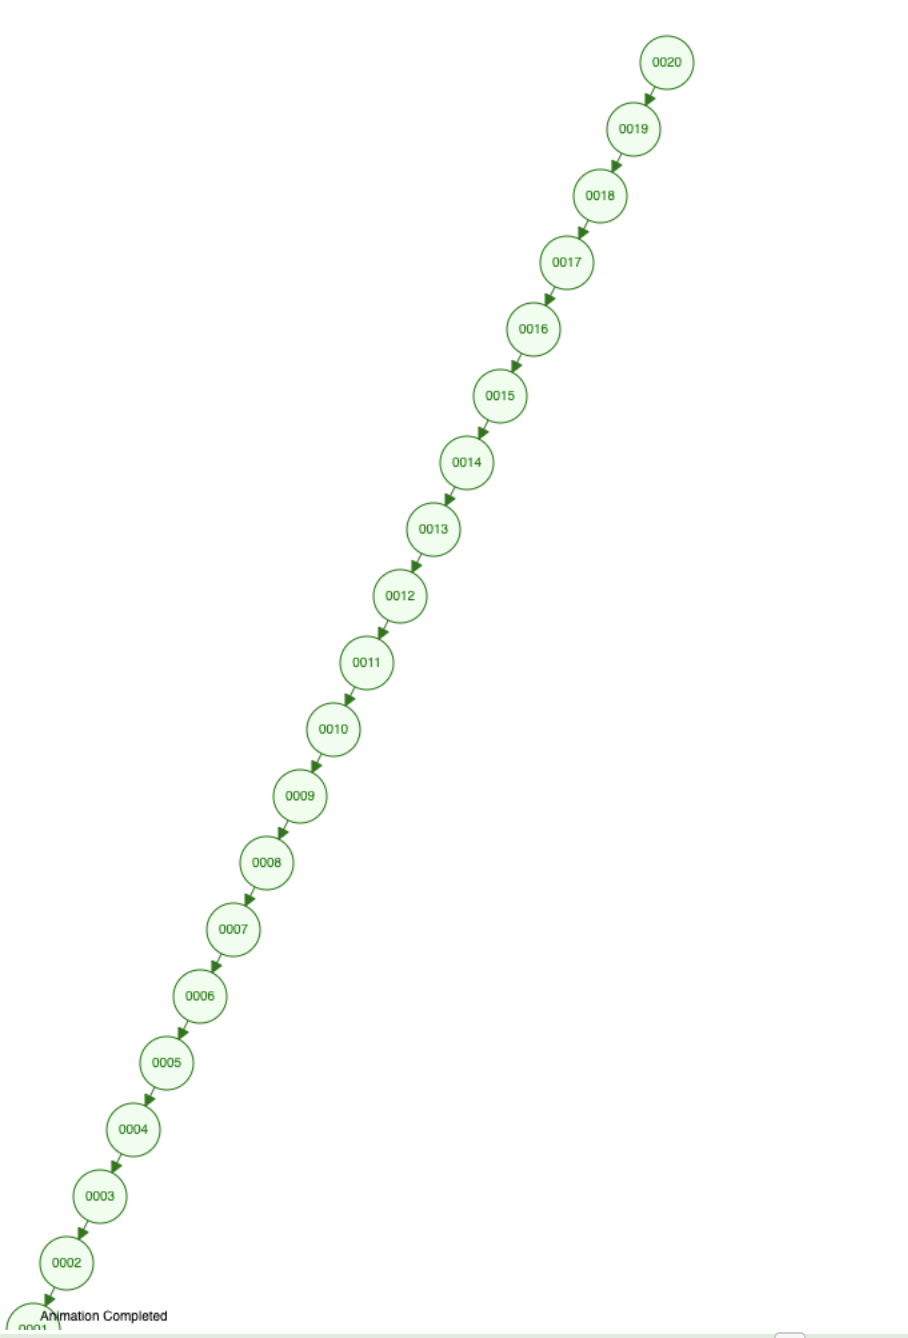
\includegraphics[scale=.5]{arbol1}
\caption{Árbol cargado a la izquierda}
\end{figure}

\center
\begin{figure}[h]
\includegraphics[scale=.5]{arbol2}
\caption{Árbol balanceado}
\end{figure}

\end{document}